\documentclass[english]{tktltiki}
\usepackage[pdftex]{graphicx}
\usepackage{subfigure}
\usepackage{url}
\usepackage[usenames,dvipsnames]{xcolor}
\usepackage{listings}
\begin{document}
%\doublespacing
%\singlespacing
\onehalfspacing

\lstdefinelanguage{Ini}
{
    basicstyle=\ttfamily\small\singlespacing,
    columns=fullflexible,
    morecomment=[s][\color{Orchid}\bfseries]{[}{]},
    morecomment=[l]{\#},
    morecomment=[l]{;},
    commentstyle=\color{gray}\ttfamily,
    morekeywords={},
    otherkeywords={=,:},
    keywordstyle={\color{red}\bfseries}
}

\title{Browsing the web and playing games using an eye tracker: practical issues}
\author{Liangyi Luo, Tomi Simsiö, Jiri Hamberg }
\date{\today}

\maketitle

\numberofpagesinformation{\numberofpages\ pages + \numberofappendixpages\ appendices }
%\classification{\protect{\ \\
%x.x [Human-centered computing],\\
%x.x.x [Interaction design]}}

\keywords{Video-based eye tracking technologies, eye controlled web browsing and gaming, practicality }

\begin{abstract}

Eye tracking technologies, albeit being about a century-old, is particularly interesting as a type of interface technology. Video-based eye tracking technologies is a branch of technology that has been proved quite useful in many fields of scientific researches as well as in daily activities. The ideas of using video-based eye tracking technologies in web browsing and playing games has been presented and discussed in recent years, and indeed, those ideas are fascinating. Introducing eye tracking technologies to those two omnipresent and extremely popular applications could open the door to richer experiences and more design possibilities. However, there are latent practical issues that reduce the applicability of video based eye tracking technology to these domains. In this report, we intend to present our project which not only verifies the practicality of aforementioned ideas but explores the relative issues in detail.   


\end{abstract}

\mytableofcontents




\section{Introduction}

This is the report on the project about eye tracking technologies for the course Interface Technologies in the Autumn of 2015. In this report, we present our project that intends to demonstrate the concepts and explore issues of using eye tracking technologies to augment gaming and web browsing experience.  

The model of the eye tracker used is Mirametrix S2. The technology Mirametrix S2 based on is called Infrared Pupil-Corneal Reflection Tracking (IR-PCR), which is one of the most widely used video-based eye tracking technologies. 

In Section 2, there is a succinct introduction to video-based eye tracking technologies in general as well as idiosyncrasies of IR-PCR in the first place, which is followed by a brief review of existing applications of eye tracking technologies. Then in Section 2, known advantages and problems of the IR-PCR technology will be briefly discussed. Lastly, there is an overview of the composition of the test platform used in the project.

There were two subjects of interest in the project, thus two program prototypes were made: a Google Chrome extension and a game controller framework.  Both prototypes used the eye tracker as the input hardware.

Section 3 reports the Chrome extension and Section 4 reports the game controller framework. In both Section 3 and Section 4, the motives and ideas for applying an eye tracking technology (IR-PCR in the project) to the corresponding interface will be elaborated in the first place. Then, there will be a brief introduction to the composition and working principle of the prototype. This is followed by an illustration of usage with some skatchings/screenshots. 

In Section 5,  an analysis on practicality of using IR-PCR technology for web browsing and for controlling game is presented. Eventually, we summarise what we have learnt during the course, then we conclude the project.


\section{Video-based eye tracking}

\subsection{A brief introduction to video-based tracking}

On the retina of a human eye, there is a small pit-shaped structure called "fovea centralis", where the density of cone cells is significantly higher than the rest of the retina. Cone cells enable a human's colour vision in well illuminated environments. Fovea centralis grands the sharp central vision, whereas the rest of retina provides much less sharp peripheral vision. The visual field of a normal human being is more than one hundred and eighty degrees, in which the fovea centralis covers about one degree only. A human has to move its eyes thus move the point of regard in order to acquire clear vision from multiple directions. Therefore, images of eye movements can be used to track a human's points of regard.

Video-based eye tracking technologies use images of eyes as raw data to compute the corresponding points of regard. A video-based eye tracking system usually consists of a camera as the input hardware and a computer system with adequate software that measures relative rotational motions of eyes from images captured by the camera. Usually, the displacements of pupils are used to infer eyes' relative rotational motions, which can be mapped to movements of points of regard through a calibration process. 

The performance of a video-based eye tracking system is limited by both the hardware and software. The camera is the most important component in an eye tracking system. The maximum resolution of the images captured by the camera determines maximum precision of measurements of eye movements. Moreover, the maximum frame rate determines the sample rate of eye movements. The sample rate is important because human eyes have rapid micro movements called "saccades" when gazing at something. Smoothing techniques are required to acquire the point of regard from saccades. Higher sample rate of saccades provides richer data for smoothing thus facilitate tracking the point of regard. As for the software, essential tasks for tracking eye movements, such as the calibration, computation, as well as some error compensations are all crucial as well. If the input hardware, id est camera, is sufficiently good, then the software has to be robust enough to report coordinates of the estimated points of regard correctly and fast.


\subsection{Infrared Pupil-Corneal Reflection Tracking}

Infrared Pupil-Corneal Reflection Tracking (IR-PCR) is one of the most popular eye tracking technologies. IR-PCR eye trackers shoot infrared light towards human eyes then use the reflection to track eye movements. There are two alternatives of IR-PCR: bright pupil tracking and dark pupil tracking. A "bright pupil" eye tracker's camera is on the path of the reflection, such that the infrared light reflected back from the retinas will enter the camera lens. In the images captured by the camera, the pupils are illuminated and appear to be bright white discs. A "dark pupil" tracker's camera avoids the path of the retinal reflection, such that the pupils are darker than irises and limbi and appear to be dark discs. Either way, the pupils are highlighted and rendered easier to track. In addition to highlighted pupils, corneas of eyes reflect the infrared light source as bright light spots, despite the position of eyes, due to corneas' hemisphere shape. Using the bright spot as reference objects, the relative motions of pupils can be measured, hence the eye movements are tracked.


\subsection{A review of applications}

There are plenty applications of eye tracking technologies. Generally speaking, an application may use eye trackers for interactions or merely observations. The former case is more often seen in human-computer interactions whereas the later is in studies and researches. 

According to users' awareness of and control over the tracking process, applications of eye tracking can be put into four categories according to Majaranta and Bulling.\cite{majaranta14}

The first category is called "explicit eye input", where a user interacts with an interface by voluntary control using gazing, blinking, or even head movements, given that some device can track head movements. In this category, some applications use only eye-based control for special cases while other implement multimodal control to avoid the "Midas touch" problem \cite{Velichkovsky97}

On the "eye-based only" side, some interesting applications are: interfaces featuring gaze gestures\cite{Drewes:2007:ICU:1778331.1778385}\cite{Ohno:1998:FEG:786112.786297}; a "hand-free" web browser\cite{5090980}; a gaze-based text input\cite{wardmackay2002}, which can achieve an input rate of 29wpm; a smartwatch interface\cite{Hansen:2015:GIT:2800835.2804332}. "Eye-based only" control technology is generally useful in scenarios where using hands are not an option. It is extremely beneficial for people with physical disabilities in hands or arms. 

On the multimodal side, some interesting applications are: multi-modal user interface\cite{538404}\cite{maglio2000}; gaze controlled games\cite{Isokoski:2009:GCG:1667488.1667491}. 

The second category is called "attentive user interfaces", where a user does not issue gaze-based commands over interfaces directly, nonetheless the system will still react to users' eye movements. Some interesting applications are: interactive movies\cite{doi:10.1080/14626260500476523}; interactive stuffed-toy\cite{Yonezawa:2007:GBS:1322192.1322218}.

The third category is called "gaze-based user modeling", where the goal is to discern patterns of user behaviors on an interface, or to assess an interface by doing so. Interesting applications are mostly researches in human-computer interaction, human cognition, or psychology. Some examples are: usability research in human-computer interaction \cite{Poole05eyetracking} \cite{Jacob2003573}; visual perception research\cite{John2004}.

The fourth category is called "passive eye monitoring". This is the case in which data of eye movements are collected for study or inspection. There is no interaction in the process. No connection between eye movements and an interface will be established. An interesting example is about tests on whether a driver is intoxicated during driving by monitoring eye movements\cite{Busloff1993}. It is worth noticing that tests are not conducted with a digital eye tracker but a simple scale and naked eyes of the tester, which marks this as one of the simplest forms of eye tracking "technology" (techniques actually).

We have found also concrete examples of applications, those in gaming control were especially interesting since one of our alternative idea for the project is about gaze controlled games. Videos of these examples can be found in the appendix. 

\subsection{Advantages and problems in using an IR-PCR eye tracker}

The Mirametrix S2 we are working with is a "bright pupil" IR-PCR eye tracker. Because an IR-PCR eye tracker generates its own reference points for tracking eyes, it does not require a user's head to remain absolutely motionless. Certain levels of flexibility on head movements is allowed. Besides, a binocular eye tracker that tracks both eyes of a user may be able to output data on users' head position based on the relative position of two eyes. The Mirametrix S2 eye tracker series happen to have this capability. This suggests that there is potential in using head gestures such as tilting head to enrich the means of control over the interface. 

On the latent problems of "bright pupil" eye tracker. Such eye trackers, which rely on the "bright pupil effect" to work, may perform differently on different individuals, due to the reason that the "bright pupil effect" isn't the same on every human \cite{Nguyen:2002:DIB:507072.507099} There could exists an inconsistency on tracking accuracy from different users even with the same device and calibration process. This actually agrees with our initial test on the Mirametrix S2 eye tracker. Considering this latent problem as well as the potentially wide user groups of the application, the software end of our system should has high error tolerance.

We are going to face some common problems of video-based eye tracking technologies too. The toughest nut might be the "Midas touch" problem.\cite{Velichkovsky97} In a "eye-based only" browser or game control system, "Midas touch" may result in unwanted operations. A possible countermeasure is using gaze gestures. \cite{Ohno:1998:FEG:786112.786297} However, more complicated gestures are needed to bring greater variations in control inputs, yet complicated eye gestures are not natural and bring fatigue. Moreover, an eye tracking device needs to be specifically positioned in order to perform with best possible accuracy. This can be problematic for laptop users.  Furthermore, calibration is required every time before use for every user. This isn't ideal for a browsing application that will be used often. Besides, there are several relatively minor problems. Users who wear spectacles or has droopy eyelids may find an eye tracker difficult to use. Some eye trackers might be sensitive to ambient light. 

\subsection{An overview of the system composition}

Our system consists of a Mirametrix S2 eye tracker as the input hardware, a virtual machine (server) with Windows OS and the system software for the eye tracker as the backend software, two program prototypes: Google Chrome plug-in and game controller framework as the frontend software, and a separate monitor as the output hardware. The software part of the system runs on a laptop (both programs were verified to work on a Linux laptop).

The Mirametrix S2 used for the project is an IR-PCR eye tracker. The official specification states that it has accuracy of less than one degree of visual angle. The "data rate" is 60Hz, means it captures an image of eyes, compute coordinates, and output x,y coordinate as floating points in range [0,1] 60 times per second. It is capable of binocular tracking, which suggests that tilting heads can be detected. It allows head motion in a 25cm width , 11cm height window with 30cm depth. The recommended distance between a user and the device is 65cm. That gives us 50cm to 80cm distance flexibility in a 25x11cm window. 

The software suit provided by the device manufacture, of which the server software and the driver are most crucial, runs only on Windows machines (including virtual machines). Hence aforementioned Windows virtual machine was used as the server that streams coordinates as data from the eye tracker. With the server running, we can communicate with it using TCP/IP protocal from a computer with operating systems other than Windows. In the project, the laptop used, which is also the host computer of the virtual server, is a Linux computer. Two program prototypes runs on Linux OS while the backend software of the eye tracker runs on a Windows virtual machine (the eye tracker server).

Through some initial test of the device, we realized that the accuracy stated in the device specifications, presumably achieved in controlled tests, was not our case. This actually agreed with what we had learned about accuracy of eye trackers in practice from literature. \cite{majaranta14} However, possible bad accuracy should be taken into account if using an eye tracking technology in daily casual activities such as web browsing and playing games is the goal. 


\section{The implementation for web browsing: a Google Chrome browser plug-in with an eye tracker}


\subsection{The motives and ideas for the interface}  

In a searching task, in which a user is browsing through large amount of web pages to find something, it will be convenient if the user can preview a web page with a given link because the link might not contain enough information to indicate the interestingness of the corresponding web page. Moreover, the user might need to constantly switch between selecting and viewing, which requires mouse input, and text entering, which requires typing with both hands on a keyboard. According to the Keystroke-level modal\cite{Card:1980:KMU:358886.358895}, pointing, selecting, and homing of using a mouse take time.

Based on the premises and assumptions above, what we can think of is a browsing mechanism that uses an eye tracker instead of a mouse as a pointing device. Besides, it has a preview function that opens a preview windows for the link the user pointed at. Therefore the project focus on the idea of pointing and previewing using an eye tracker.  



\subsection{The composition and working principle of the plug-in}

The browser plug-in is composed of three main components. The Mirametrix server, provided by Mirametrix alongside the hardware and driver packages, communicates directly with the eye tracking hardware through the Windows driver. The Mirametrix server exposes the Open Eye Tracking API through a HTTP server. The API is built using XML encoded messages.

We built a websocket server to parse the XML data stream from the Mirametrix server and to pipeline the data in JSON format to our browser plug-in. The websocket protocol was chosen as the communication protocol between the websocket server and the plug-in since it is lightweight, reliable and highly supported protocol in the domain of web browsers. The websocket server spawns a thread for each connecting client. The thread requests data from the Mirametrix server and then listens for incoming data until disconnected. The thread serializes the TCP byte stream at XML message boundaries and sends these to the plug-in in JSON format using the websocket protocol.  

Finally, we decided to build the web browser plug-in using Chrome browser because the developer tools of the Chrome browser were familiar to the majority of our team. The plug-in connects to the websocket server and register a handler for incoming websocket data frames. Each frame consists of the user's current gaze fixation x,y-coordinates. These coordinates are then transformed from the screen coordinates to window coordinates of the browser. The plug-in will then search the DOM for the first hyperlink element whose bounding rectangle contains the received x,y coordinate and will open a pop-up window displaying a preview of the hyperlink's destination if such hyperlink element was found.

Figure \ref{pluginarchitecture} illustrates this architecture and layout of the components.

%{illustration}
\begin{figure}[h]
\begin{center}
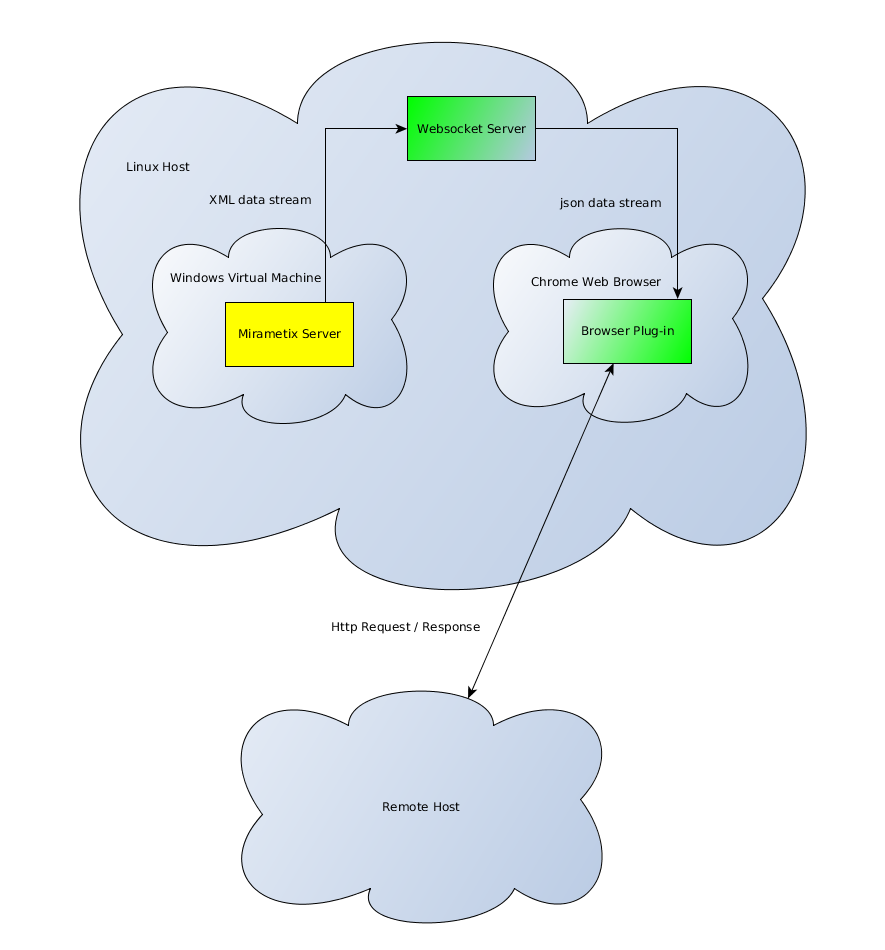
\includegraphics[width=0.6\textwidth]{plugin_architecture.png}
\caption{High level architecture and layout of the browser plugin. Green rectangles represent components that we implemented.}
\label{pluginarchitecture}
\end{center}
\end{figure}

\subsection{An illustration of the usage of the interface}

To use the eye tracking interface, the user navigates to a web page of his/her choice using the Chrome browser. The user then activates the eye tracking plug-in by clicking on the plug-in icon with two nested black circles. A blank pop-up window will open. After the pop-up window is opened, whenever the user gazes at a link for a while, a preview of that link's destination will be opened to the pop-up window. Figure \ref{pluginusage} shows the plug-in in action. To use the plug-in, the user must first make sure that the Mirametrix HTTP server is running in a Windows virtual server. After this, the websocket server must be started by issuing \verb|python ws_server.py| command. After this initial set up, the user can start the Chrome web browser and run the plug-in as instructed above.

%{illustration}
\begin{figure}[h]
%\begin{figure}[tbh] t= top, b = bottom, h=here
\begin{center}
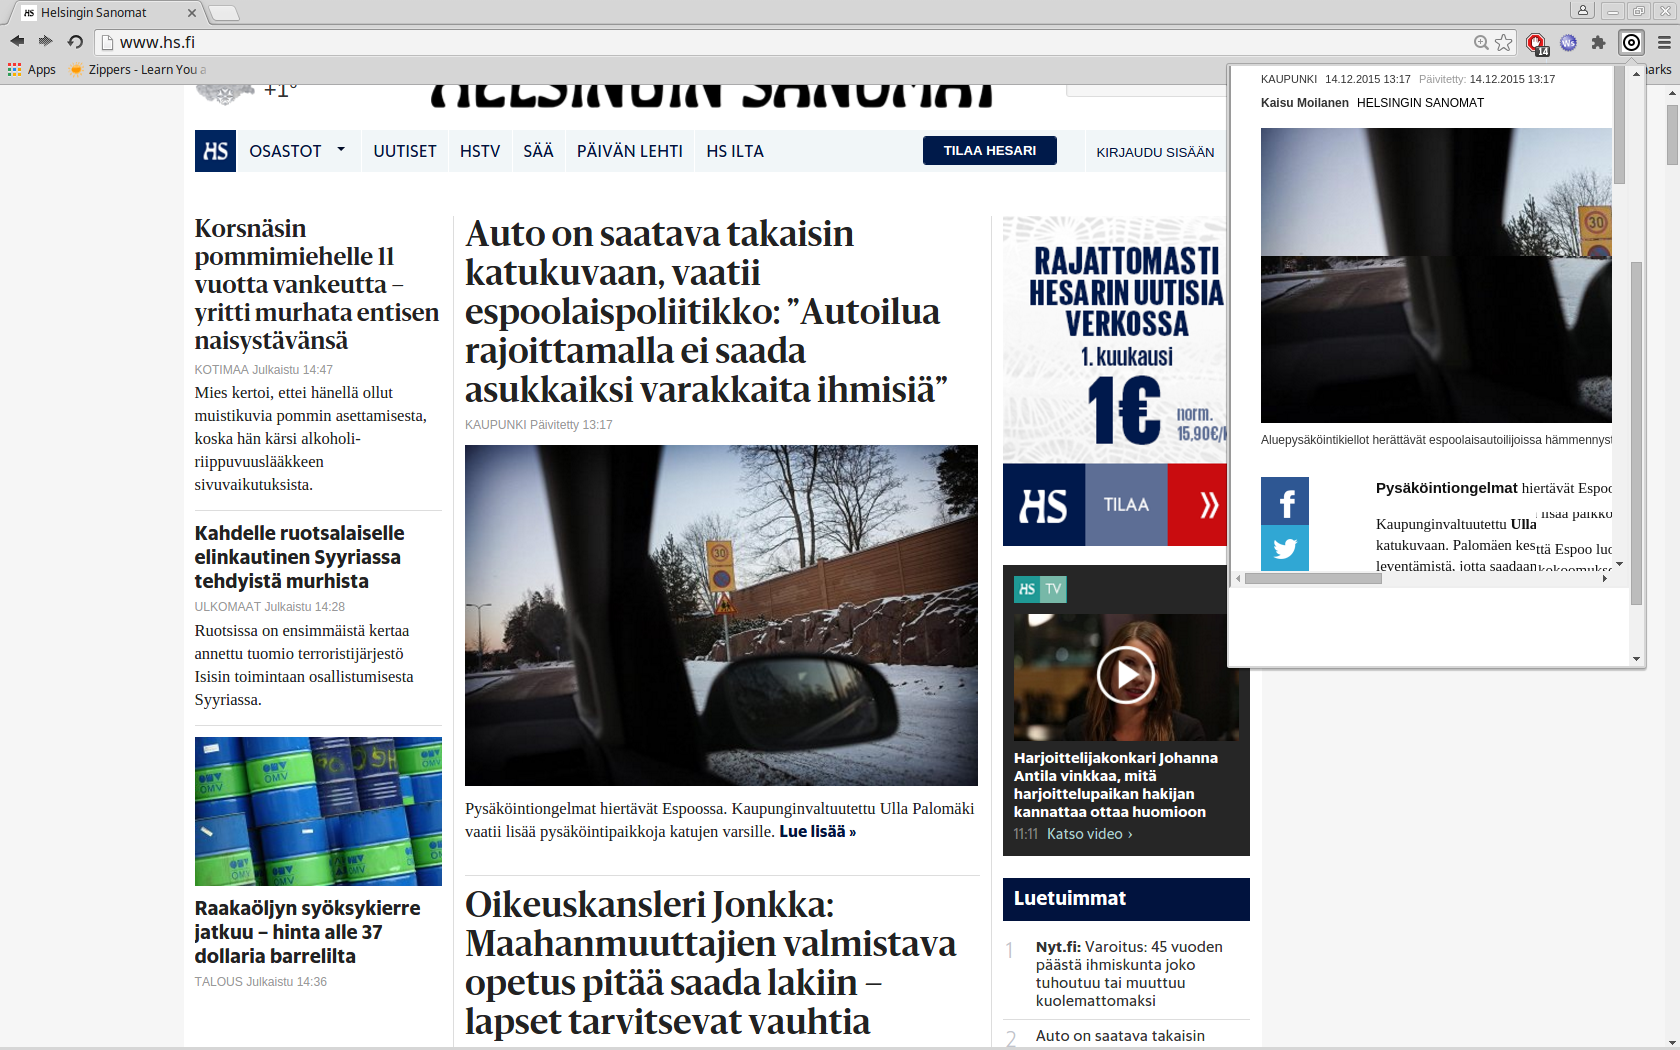
\includegraphics[width=0.9\textwidth]{browser_plugin.png}
%\rotatebox{90}{\includegraphics[scale=.75]{kuvaesimerkki.pdf}}
\caption{Using the browser plug-in to display previews of news articles by gazing at the link.}
\label{pluginusage}
\end{center}
\end{figure}

%\pagebreak


\section{The implementation for gaming: Using an eye tracker as a game controller}


\subsection{The motives and ideas for the interface design}

Certain genres of games such as Simulation and Real-Time Strategy (RTS) requires navigating the view window/camera towards different directions of the map. This is traditionally done by a clicking or moving mice or press arrow keys. With an eye tracker, we might explore more possibilities in keyboard-and-mouse control if hands are freed from view field navigation tasks. Besides, using eye trackers might help play Simulation or RTS games on game consoles.


\subsection{The composition and working principle of the game controller framework}

Our game controller framework aims to provide easily configurable camera-movement controlling for all games that have a camera, which is moved by either arrow-keys or WASD-keys. When the user looks to a side of the screen, our controller framework emulates keyboard keypress to move camera in that direction. For example, when the user looks to close of the left border of the screen, our framework emulates left arrow or A-key press to move the camera leftwards. Keypress emulation is done via the uinput kernel module.

Every game has different 2D user interface and thus every game needs a different configuration to specify when and how to move the camera. This is done in our framework with game-specific configuration files. Listing \ref{gcfconf} is an example of such file.

We got up to 60 gaze-events per second from the eye tracker each telling where this user is looking at that moment. We reference to these events as ticks. The first configuration variable \verb|ticks_needed| defines how long the user needs to look at the side of the screen before the camera is being moved. The second variable \verb|action_every_ticks| specifies how many ticks to wait between emulated keypresses when the user keeps looking at the side of the screen. The movement happens by either arrow or WASD-keys, defined by the \verb|move_method|-variable.

The \verb|*_start| and \verb|*_margin|-variables define where the user needs to look in order to move the camera. The values are percentages of the screen. Horizontally left border of the screen is 0 and right border is 1. Vertically top border is 0 and bottom border is 1. So for example \verb|left_start = 0.2| means that when user is looking at somewhere on the leftmost fifth of the screen, the camera is being moved left. The \verb|*_margin|-variables may be helpful to rule out some possible 2D UI-bars on the sides of the screen. \verb|left_margin=0.0|, \verb|right_margin=1.0|, \verb|up_margin=0.0| and \verb|down_margin=1.0| means that no margins are in use.

\bigskip
\begin{lstlisting}[language={Ini},caption={Example of game-specific configuration file},label={gcfconf}]
[Camera]
# Number of subsequent ticks needed to make action
ticks_needed = 1
# How many ticks to wait between actions
action_every_ticks = 1
# How to move the camera? 'wasd' or 'arrows'
move_method = wasd

# Points when to start moving camera
left_start = 0.2
right_start = 0.8
up_start = 0.2
down_start = 0.75

# Reserve a margin where eg. infobars are
left_margin = 0.0
right_margin = 1.0
up_margin = 0.0
down_margin = 0.9
\end{lstlisting}
\bigskip

The game controller framework is used with command \verb|python main.py|. This lists all available game configurations. Controlling can be started with e.g.\newline \verb|python main.py -g cities_skylines|.

\subsection{An illustration of the usage of the interface}

Figure \ref{citiesskylines} illustrates where the user needs to look while playing Cities: Skylines with configuration from listing \ref{gcfconf}. Camera will move up while looking at the top red area, down while looking at the bottom red area and sideways while looking at the blue areas. Vertical an horizontal movement can happen simultaneously. Cities: Skylines has a toolbar on the bottom of the screen, so that area is ruled out by setting \verb|down_margin=0.9|.

\begin{figure}[h]
\begin{center}
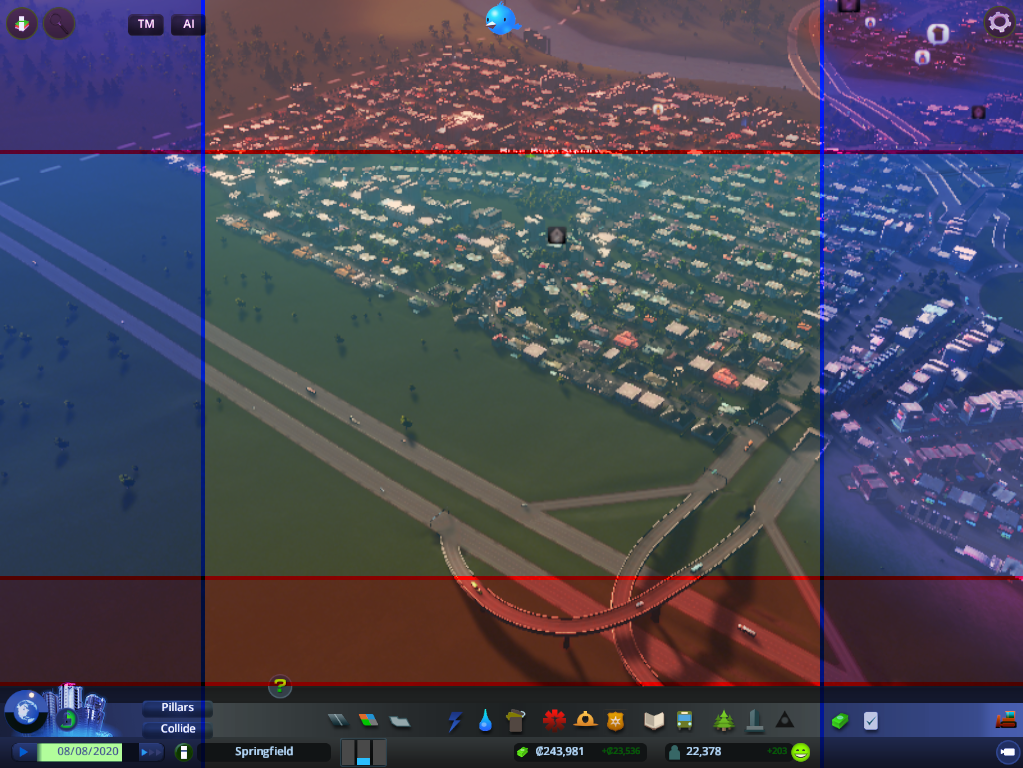
\includegraphics[width=1\textwidth]{cities_skylines.png}
\caption{Relevant screen sections highlighted over a screenshot from Cities: Skylines}
\label{citiesskylines}
\end{center}
\end{figure}



\section{Discussion}

\subsection{Practicality analysis}

First, accuracy is the cornerstone of any eye tracking based interface. In the project, accuracy issues were major issues in both prototypes. In the test of the Chrome extension, the test subject had difficulties in pointing at links with small icons. In the test of the game controller framework, navigating upwards did not work well. This wasn't so surprising since our early test had already exposed the problem of pointing accuracy. 

On the negative side, insufficient pointing accuracy could be a bigger issue in practice given that the position and calibration of an eye tracker could be worse than the condition in our test. Consequently, inaccuracy leads to the requirement for bigger clickable logos in web browsing. Besides, inaccurate pointing may result in unwanted previewing or opening the wrong web page. This may be more or less an issue that depends on the specific browsing task. For controlling games, less accuracy means less available operations for eyes to commence. Because most pointing operations in games are originally based on mouse pointing or at least joystick pointing, both are more accurate than current eye trackers.

On the positive side, inaccuracy issues are device dependent, suggesting that "eye pointing" can become more practical after better eye tracking technologies are developed. Therefore, how well can the idea of using eye trackers in web browsing or controlling game be realised is relying on the advancement of eye tracking technologies. 

Otherwise, we can think from a different angle. Even if the accuracy of current eye tracking technologies can hardly be improved, the interfaces of the relative applications can adapt. A reference case for web browsing is that many websites provide web pages customised for small screens of mobile phones. However, the current situation for eye trackers is different from mobile phones. Eye tracking technologies are not required for most browsing tasks and it is even harder to find a case where eye trackers are absolutely necessary. Expecting eye trackers to become as ubiquitous as mobile phones is unrealistic. Likewise, games that use eye trackers are minority because most players are content with mice, keyboards, and joysticks and there hasn't been a case in which the need for eye trackers is rigid. Nevertheless, there might be more hope to see a burgeoning use of eye trackers in games because eye trackers indeed have the potential to provide interesting features in games such as "eye contact with non-player characters". Most importantly, such features in games might work with compromised accuracy.

Second, the practicality of using an eye tracker in web browsing or controlling games depends on how things are done exactly. Certain details are crucial. Given the same idea and equipment for an interface, details in the implementation determine the user experience, hence the relative optimisation is important. In our tests, the delay before opening a preview or navigating towards a direction was a detail that required attention. We used semi-arbitrary values according to our intuitions; however in practice, researches and experiments were done in order to optimise an interface with regard to details.

Third, there is no perfect practicality. Some inevitable and technology-specific problems in using the device were expected at the beginning of the project. We commenced calibrations before each test and the body of the test subject needed to remain near motionless during the test. If there existed a calibration-free eye tracker with a large reception field, we could have kept the prototypes devoid of such problems for sure; but other problems, such as high cost and large size, might pop up. Therefore, before an interface with eye trackers is designed for practical use, it is very crucial to discern the inevitable problems of each optional eye tracking technology, weigh advantages of each technology against its disadvantages, then choose prudently. Possible trade-offs should be expected.

Last but not least, practicality is not absolute. It depends on also the requirements of the relative application. Why we found our eye tracker being not practical in our project was partially due to the high requirements on the accuracy of the pointing device in both web browsing and playing games. In addition, both applications would like to avoid incommodious procedures such as calibrations and staying motionless. Considering the existing wide range of uses of eye tracking technologies, it is safe to infer that eye trackers are impractical in some applications does not suggest that they are impractical in other applications. In order to make eye trackers more practical in an application, either improve the device or lower the requirements of the application. The later approach could use some creativity. The aforementioned idea of "eye contact with NPCs" in games is a good example. 

All in all, there are three major factors affect the current practicality of eye trackers. The first is that eye tracking technologies are still very far from ideal. The second is the optimisation done for an interface with eye trackers. The third is that current eye trackers may or may not meet the requirements of an intended application. In addition to the three factors listed above, it is worth mentioning that users may also play an important role. How do human eyes really work is not necessarily intuitive for users with no relative backgrounds, hence matching the expectations of these users. Users might need to know that they can not point with an eye tracker like with a mouse, even if there existed a perfectly accurate eye tracker. Therefore, users might need some "get-used-to" before an eye tracker can become really useful. 

%We might not need this part because repetitive contents.
\subsection{Things we learned}

The eye tracking technology is applicable to a wide spectrum of interesting topics in human computer interaction. However, great care must be taken in designing and evaluating an eye tracking interface as well as the eye tracking hardware as these may be subjects to many subtle sources of undesirable effects. It would appear, based on our experience working on this project, that the eye tracking technology of today is most practical as a secondary source of input and that interactions requiring great precision should be implemented using other modalities.


\subsection{Conclusion}

We have demonstrated, with our two prototypes, how eye tracking interfaces can be used to enrich our every day activities such as browsing the web or playing computer games using existing games and web browsers. The practicality of our prototypes is heavily constrained by the available time, our lacking expertise with the technology as well as the constraints of the eye tracking hardware. We hope that our work may inspire others to explore the practical applications for this underutilized technology.
      

%\enlargethispage{5mm}

%\subsection{}

%\subsection{}

%\enlargethispage{5mm}



%\nocite{*}
\bibliographystyle{tktl}
\bibliography{lahteet}

\lastpage

\appendices

\pagestyle{empty}

\internalappendix{1}{Videos about eye tracking applications}

Most videos feature Tobii devices due to the fact that Tobii is one of the major eye tracking device manufactures.

"BMX rider Stephen Murray controls his computer with only his eyes"
https://www.youtube.com/watch?v=b\_wsnc8IdCQ

"Demo of Tobii EyeX in Gaming"
https://www.youtube.com/watch?v=oSo8fbZfHLk

"Gaze control of StarCraft2"
https://www.youtube.com/watch?v=s4ZCQ-jZxyE

"Tobii Gaze Interface for Windows 8 Revolutionizes Computer Interaction"
https://www.youtube.com/watch?v=3MoGzTdQnX8

\end{document}


